\documentclass{article}
\usepackage{anyfontsize}
\usepackage{lmodern}
%\usepackage{extsizes}
\usepackage[utf8]{inputenc}
\usepackage{multicol}
%\usepackage{parskip}
\usepackage{amsmath}
\usepackage{titlesec}
\usepackage{enumitem}
\usepackage{graphicx}
\usepackage{ulem}
\usepackage{xcolor}
\usepackage[printwatermark]{xwatermark}
\usepackage[letterpaper, portrait, margin=0.1in]{geometry}
\usepackage{titlesec}

% \newwatermark[allpages,color=gray!35,angle=45,scale=3,xpos=0,ypos=0]{nwalter2}


\title{CS 425 Final Cheat Sheet}
\author{nwalters512 }
\date{December 2018}

\titleformat*{\section}{\small\bfseries}

\titlespacing*{\section}{0pt}{0ex}{0ex}
\setlist{partopsep=-\parskip,parsep=0pt}

\begin{document}
\fontsize{7}{7}
\selectfont
\begin{multicols*}{3}
\section{Distributed systems}
\textbf{Examples}: client/server, the web, the internet, DNS, Gnutella, BitTorrent, ``cloud", NCSA, AWS datacenter \\
\textbf{Definitions}: ``A collection of independent computers that appear to the users as a single computer", ``Several computers doing something together", ``A distributed system is a collection of entities, each of which is autonomous, programmable, asynchronous and failure-prone, and which communicate through an unreliable communication medium." \\
\textbf{Goals}: heterogeneity, robustness, availability, transparency (hides internal workings from users), concurrency, efficiency, scalability, security, openness

\section{Clouds}
\textbf{Types}: public (provide services to any paying customer) or private (accessible only to company employees) \\
\textbf{Benefits}: save time and money! \\
\textbf{Definition}: Lots of storage + compute cycles nearby \\
\textbf{Single-site architecture}: compute nodes grouped into racks; switches connecting racks (both top-of-rack and core); hierarchical network topology \\
\textbf{History}: first datacenters (1940s to 1960s), timesharing and data processing companies (1960s to 1980s), grids (1980s to 2000s), clusters (1980s to present), clouds and datacenters (2000s to present) \\
\textbf{Doubling periods}: storage (12 months), bandwidth (9 months), CPU capacity (18 months) \\
\textbf{Modern cloud features}: massive scale, on-demand access, data-intensive nature, new programming paradigms (MapReduce, Hadoop, NoSQL) \\
\textbf{WUE}: $\frac{\text{Annual water usage}}{\text{IT equipment energy}}$ - low is good \\
\textbf{PUE}: $\frac{\text{Total facility power}}{\text{IT equipment power}}$ - low is good \\
\textbf{``As a service"}: hardware (barebones machines), infrastructure (AWS, Azure), platform (Google App Engine), software (Google Docs) \\
\textbf{Data-intensive computing}: Network/disk I/O more important than CPU utilization \\
\textbf{Academic clouds}: Emulab, PlanetLab \\
\textbf{Public research clouds}: needs grant; Chameleon Cloud, CloudLab

\section{MapReduce}
\textbf{Map}: parallelly process lots of records to generate key/value pairs \\
\textbf{Reduce}: processes and merged intermediate values per key; partitions keys for parallelism (shuffle) \\
\textbf{Sorting}: Map output sorted with quicksort, reduce input sorted with mergesort \\
\textbf{Filesystems}: map input (distributed), map output (local), reduce input (multiple remote disks to local), reduce output (distributed) \\
\textbf{YARN}: global Resource Manager (scheduling), per-server Node Manager, per application Application Master (negotiates with RM and NMs, detect failures) \\
\textbf{Locality}: HDFS stores 3 replicas of each chunk (2 on one rack, 1 on another); MApReduce tries to schedule a job on a) a machine with a replica of input, b) on the same rack as a machine with replica of input, or c) anywhere

\section{Gossip}
\textbf{Multicast}: disseminates message to group of nodes; nodes can crash and packets can be dropped; protocol should be reliable (atomic, 100\% delivery) and fast \\
\textbf{Centralized}: slow ($O(n)$ time to broadcast) and not fault-tolerant (what if sender failed halfway through sending?) \\
\textbf{Tree-based}: build spanning tree; failed nodes may not pass on message until tree is repaired; tree maintenance is hard; ACK/NAK floods could occur; (REWATCH BEFORE SEPT 11 SRM/RMTP) \\
\textbf{Gossip}: periodically picks $b$ random nodes and sends messages to them; needs deduplication; all nodes start sending messages as well once ``infected" \\
\textbf{Push gossip}: start gossiping after receive message; if multiple messages, gossip random subset, or recently-received, or higher priority; lightweight in large groups, spreads quickly, fault-tolerant \\
\textbf{Pull gossip}: poll randomly selected processes for new messages \\
\textbf{Infection}: continuous time process
$$x_0 = n, y_0 = 1, \dfrac{dx}{dt} = -\beta x y$$
$$x = \dfrac{n(n+1)}{n+e^{\beta(n+1)t}}, y = \dfrac{(n+1)}{1 + ne^{-\beta(n+1)t}}$$
\textbf{Epidemic multicast}: $\beta = b/n$, so at time $t=c\log{n}$,
$$y = (n+1) - \dfrac{1}{n^{cv-2}}$$
So, within $c\log{n}$ rounds [low latency], all but $\frac{1}{n^{cb-2}}$ have received the message [reliability] and each node has transmitted no more than $cb\log{n}$ messages [lightweight] \\
\textbf{Fault tolerance}: Packet loss (50\% loss, analyze with $b$ replaced with $b/2$, takes twice as many rounds for same reliabiltiy), node failure (50\% fail, analyze with $n/2$ and $b/2$, same as above) \\
\textbf{Pull vs. push}: for both, takes $O(\log{N})$ rounds for $N/2$ to get gossip; after first half, pull is faster, as it takes $O(\log{\log{N}})$ time \\
\textbf{Topology-aware}: for random selection, core routers face $O(N)$ load. Fix: pick target in your subnet $i$ with probability $1-1/n_i$.

\section{Failure detection}
\textbf{Goals}: scalable (equal load per member), fast (time until some process detects failure), complete (each failure detected), accurate (no mistaken detection); impossible to have both accuracy and completeness (or could solve consensus!) \\
\textbf{Preferred}: Guaranteed completeness, partial accuracy guarantee
\textbf{Centralized heartbeating}: all ping one node, if no ping from $p_i$ received within timeout, declare $p_i$ failed. Bad: $O(N)$ load on central node \\
\textbf{Ring}: ping neighbors. Unpredictable on multiple simultaneous failures \\
\textbf{All-to-all}: equal load per member, but a single heartbeat loss means a false detection \\
\textbf{Gossip}: nodes periodically gossip membership list to random nodes; on receipt, merged with local membership list; member marked as failed when entry times out, deleted after cleanup period to prevent ghost entries \\
\textbf{Analysis}: heartbeat takes $O(\log{N})$ time to propagate, so $N$ heartbeats take $O(\log{N})$ time to propagate for $O(N)$ bandwidth per node, $O(N\log{N})$ time for $O(1)$ bandwidth, $O(\frac{N}{k}\log{N})$ for $O(k)$ bandwidth. If Tgossip is decreased, bandwidth increases, detection time stays unchanged. If Tfail, Tcleanup increased, make fewer mistakes, bandwidth unchanged, detection time increases. \\
\textbf{Load}: All-to-all: $L=N/T$; gossip: $T=\log{N}\cdot t_g, L=N/t_g=N\log{N}/T$; optimal: independent of $N$! \\
\textbf{SWIM}: every period $T\prime$, $p_i$ sends ping to $p_j$; if $p_j$ ACKs, $p_j$ declared alive; if no ACK, request indirect ping from $k$ random processes \\
\textbf{SWIM detection time}: probability of being pinged in $T\prime = 1-(1-\frac{1}{N})^{N-1}=1-e^{-1}$, so $E[T] = T\prime\cdot\frac{e}{e-1}$, so complete: any alive member detects failures \\
\textbf{Time-bounded completeness}: round-robin pinging, randomly permute list after each traversal. Failure is detected in worst case $2N-1$ protocol periods \\
\textbf{Member dissemination}: piggyback on failure detector messages for infection-style dissemination; maintain buffer of recently joined and evicted processes and prefer recent updates \\
\textbf{Suspicion}: per-process incarnation number, only $p_i$ can increment $p_i$'s number; higher #s override lover #s; for given #, suspect $>$ alive, failed $>$ anything else \\
\textbf{In industry}: used by Serf/Consul, Uber's ringpop

\section{Peer-to-peer systems}
\textbf{Napster}: napster server maintains $<$filename, addres, port$>$ tuples but no files; clients upload list of files to server; client queries server for keyword, server responds with list of tuples; clients communicate with each other, selecting the best host for transfer; uses TCP \\
\textbf{Gnutella}: eliminates servers, clients act as servers too; clients connected in overlay graph; messages are routed within the overlay graph \\
\textbf{Gnutella protocol}: \textit{Query} (search), \textit{QueryHit} (response to query), \textit{Ping} (probe network for peers), \textit{Pong} (reply to ping with address of another peer), \textit{Push} (initiates file transfer); header contains unique descriptor ID, type, TTL (decremented at each hop, dropped at 0), hops (incremented at each hop), payload length \\
\textbf{Gnutella search}: flooded out, ttl-restricted, only forward once; \textit{QueryHit}s routed on reverse path \\
\textbf{Avoiding excessive traffic}: peer maintains list of recently received messages; query forwarded fo all neighbors except query source; queries forwarded only once; \textit{QueryHit} routed back only to peer from which \textit{Query} received; duplicates are dropped; \textit{QueryHit} with unseen ID is dropped \\
\textbf{QueryHit response}: requester chooses "best" responder, initiates HTTP request directly to peer, peer replies with file packets. HTTP is used (standard, debugged, \texttt{Range} header supported \\
\textbf{Firewalls}: if unable to reach peer, routes a \textit{Push} to responder and has the responder send a HTTP-like \texttt{GIV} message, requester then sends \texttt{GET} and continues as before \\
\textbf{Pingpong}: \textit{Ping} flooded out, \textit{Pong} routed along reverse path; used to update set of neighboring peers periodically \\
\textbf{Problems}: ping/pong constituted 50\% of traffic (solution? multiplex, cache, reduce frequency), repeated searches (cache \textit{Query} + \textit{QueryHit} messages), freeloaders (70\% of users in 2000), flooding results in excessive traffic \\
\textbf{FastTrack}: like Gnutella, but with supernodes! Peers become supernodes by earning reputation; supernodes store $<$filename, peer pointer$>$ like Napster; peer searches by querying supernode \\
\textbf{BitTorrent}: files split into blocks; person wanting file first gets tracker from a website, then asks tracker for peers, then gets blocks from peers \\
\textbf{Optimizations}: dowload Local Rarest Block first (early download of blocks that are least replicated among neighbors), tit for tat bandwidth (provide blocks to neighbors with best download rates), choking (limits \# neighbors to which concurrent uploads allowed) \\
\textbf{Distributed hash table}: allows lookup, insertion, and deletion of objects (files) with keys \\

\section{Mutual exclusion}

\section{RPCs \& concurrency control}
\textbf{Local Procedure Call}: exactly-once semantics \\
\textbf{RPC Semantics}: at most once (Java RMI), at least once (Sun RPC), maybe/best-effort (COBRA) \\
\textbf{Idempotent}: applied multiple times without any side effects; can be used with at-least-once semantics \\
\textbf{Marshalling}: convert req/res into common, platform independent representation \\
\textbf{Transactions}: either comples and commits all operations, of aborts with no effect \\
\textbf{ACID}: atomic (all or nothing), consistency (if starts in consistent state, transaction ends in consistent state), isolation (transactions performed without interference from other transactions), durability (all effects saved in permanent storage after transaction completed successfully) \\
\textbf{Serial equivalence}: interleaving of transactions is serially equivalent iff some ordering of transactions which gives the same end result as the original interleaving \\
\textbf{Conflicting operations}: if combined effect depends on order of execution (R then W, W then R, W then W) \\
\textbf{Checking serial equivalence}: iff all pairs of conflicting operations are executed in the same order for all objects they both access (label all pairs $(T1, T2)$ or $(T2, T1)$, all pairs should be marked the same) \\
\textbf{Upshot}: at commit point, check for serial equivalence with all other transactions' if not equivalent, abort $T$ and roll back writes that $T$ did \\
\textbf{Pessimistic CC}: prevent transactions from accessing same object (locking; use R/W locks for better perf) \\
\textbf{Optimistic CC}: assume the best, allow transactions to write, but check later; higher concurrency and transactions per second \\
\textbf{Two-phase locking}: transaction cannot acquire or promote any locks after it has started releasing locks (growing/shrinking phase; strict: only release locks at commit point); proof of serial equivalence by contradiction (growing/shrinking phases would overlap) \\
\textbf{Deadlocks}: mutual exclusion, preemption, circular wait all necessary
\textbf{Basic optimistic CC}: check serial equivalence at commit time, roll back if abort (problem: cascading aborts) \\
\textbf{Timestamp ordering}: assign each transaction and ID; ID determines position in serialization order; ensure for $T$ a) $T$'s write to $O$ allowed only if transactions that have R/W $O$ had lower IDs than $T$, and b) $T$'s read to $O$ allowed only if $O$ was last written by transaction with lower ID than $T$; abort if violation \\
\textbf{Multi-version CC}: maintain per-transaction tentative version and committed version; each tentative version has timestamp; on R/W, find ``correct" tentative version to R/W from (tries to make transactions only R/W from ``immediately previous" transactions \\
\textbf{Eventual consistency}: form of optimistic concurrency control in K/V stores
\textbf{Cassandra/DynamoDB}: last write wins (overwrite only if new write's timestamp $>$ current timestamp) \\
\textbf{Riak}: vector clocks! Implements causal ordering, detect if a) new write is strictly newer than current value, or b) if new write conflicts with existing value. For b) \textit{sibling value} is created to be resolved by user/application; size/time based pruning to prevent clocks from getting too many/too old entries

\section{Replication control}
\textbf{Motivation}: fault-tolerance, load balancing, availability (with replication, probability of available replica is $(1 - f^k)$), transparency (client doesn't know multiple copies exist), consistency (all clients see consistent copy of data) \\
\textbf{Passive replication}: use primary replica \\
\textbf{Active replication}: treat all replicas identically; multicast inside replica group with any type of multicast ordering; handle failures with virtual synchrony \\
\textbf{One-copy serializability}: true if equivalent to a serial execution of transactions over a single logical copy of the database \\
\textbf{Transactions}: might touch object on multiple servers, need atomic commit (consensus!)
\textbf{One-phase commit}: coordinator server initiates atomic commit \\
\textbf{Two-phase commit}: coordinator sends ``prepare"; servers save updates to disk, respond with Y/N; if coordinator receives all Y within timeout, tell servers to commit updates from disk to store; otherwise, abort all
\textbf{Paxos}: server proposes message for next sequence number, group reaches consensus (or not); allows for ``no" votes

\section{Stream/graph processing}
\textbf{Motivation}: have lots of data, want high throughput and low latencies \\
\textbf{Storm}: tuples, streams, bolts, spouts, topologies (cycles possible) \\
\textbf{Bolts}: parallelize by splitting streams among multiple tasks (grouping: shuffle, fields, all) \\
\textbf{Cluster}: master (runs Nimbus, distributes codes, assigns tasks, monitors failures), worker (runs supervisor, receives work, runs executors that run groups of tasks), Zookeeper (coordinates communication, stores state) \\
\textbf{Twitter Heron}: uses backpressure, better throughput \\
\textbf{Spark}: Resilient Distributed Datasets (RDDs), immutable partitioned collections of records built through map/join/etc.; log operations and recompute lost portions if failure occurs \\
\textbf{Graph processing}: shortest paths (routing, degrees of separation), matching (dating), PageRank \\
\textbf{Algorithm}: work in iterations; each vertex gets a value; in each iteration, a vertex a) gathers values from immediate neighbors, b) does computation with own/neighbor values, c) updates value and sends to neighboring vertices (gather, apply, scatter); terminates after fixed iterations or values stop changing \\
\textbf{Processing}: assign each vertex to a server; perform gather-apply-scatter for all assigned vertices; assign based on hash or locality (assign vertices with more neighbors to same server as neighbors, reduces traffic after each iteration) \\
\textbf{Pregel}: master/worker (P2P workers); data persisted on DFS; fault-tolerance via checkpointing and recovery; fast!

\section{Scheduling}
\textbf{Goals}: throughput, high utilization of resources \\
\textbf{FIFO/FCFS}: queue in arrival order, execute when processor free (average completion time might be high) \\
\textbf{STF}: order tasks by running time, run shortest task first (optimal (minimal average completion time), can lead to starvation; special case of priority scheduling) \\
\textbf{Round-robin}: run portion of task, preempt after quantum expires, add to end of queue (preferable for interactive applications) \\
\textbf{Hadoop Capacity Scheduler}: multiple queues (possibly hierarchical), each queue contains multiple jobs; each queue guaranteed some portion of cluster capacity; elasticity (can occupy more resources if they're free; no preemption \\
\textbf{Hadoop Fair Scheduler}: goal is for all jobs to get equal share of resources; cluster divided into pool, resources divided equally between pools; configurable scheduler within pool; preemption allowed (kill most recently started tasks to minimize wasted work; OK because tasks are idempotent) \\
\textbf{Estimating task lengths}: hard; can estimate (proportional to size of input; weighted average by input size across other tasks in job) \\
\textbf{Dominant-Resource Fair Scheduling}: tries to handle multi-resource requirements (mem/CPU/etc.); jobs have resource vectors $<N \text{ CPUs}, M \text{ GB RAM}>$; for a given job, the \% of its dominant resource type that it gets cluster-wide is same for all jobs (Job 1 RAM dominant, Job 2 CPU dominant, Job 1 \% RAM = Job 2 \% CPU) \textbf{(REVIEW THIS LOL)}

\section{Structure of networks}
\textbf{Properties}: Clustering coefficient ($P(AB | (AC \&\& CB)$), path length (shortest path); Extended right graph (high CC, long paths), Random (low CC, short paths), Small world (high CC, short paths)
\textbf{Small-world resilience}: most nodes have small degree, few nodes have high degree; killing lots of random nodes won't disconnect, but a few high-degree nodes will

\section{Distrib file systems}
\textbf{Unix FS}: file descriptors (handle for process to access file); must open file before reading/writing; descriptor maintains R/W pointer to offset within file; R/W automatically advances pointer \\
\textbf{Distributed FS}: client does RPC to perform file ops; desirable properties: transparency (behaves like local FS), concurrent clients, replication (fault tolerance) \\
\textbf{One-copy update semantics}: when file is replicated, contents visible to clients are no different from when only 1 replica \\
\textbf{Client API}: read/write specifies absolute position and num bytes, position maintained by client (should be idempotent and stateless, unlike Unix) \\
\textbf{NFS}: client integrated with kernel, performs RPC to server; server allows mounting files and directories (essentially, pointers); allows processes to access file descriptors (transparency!); server caching (store recently access blocks in memory (supports locality of access)); writes: delayed (flush every 30s, fast but not consistent), write-through (write to disk immediately, consistent but maybe slow); client caching ($Tc =$ time of cache entry last validated, $Tm =$ time when block last modified at server, block valid at $T$ if $(T-T_c < t)$ or $(Tm_{\text{client}} = Tm_{\text{server}})$, delayed write to server on write) \\
\textbf{AFS}: whole file serving/caching (based on assumptions that most files accessed by single server, most files small, files read more often than written, reads typically sequential), Venus client, Vice server, optimistic reads/writes, opened files get callback promise (Vice notifies Venus if another client modifies/closes)

\section{Distrib shared memory}
\textbf{Benefit}: same code as if running on same multiprocessor OS \\
\textbf{Impl}: cache maintained at each process, stores recently accessed pages; pages mapped in local memory; on page fault, kernel invokes DSM \\
\textbf{Protocol}: Owner is process with latest version; page in R or W state; when page in R state, owner has R copy, others may have R copies, no W copies; when page in W state, only owner has copy \\
\textbf{Read}: [O?, R]: read from cache; [null, other R]: ask for copy, mark R, do read; [null, other W]: ask other to degrade to R, ask for copy, mark R, do read \\
\textbf{Write}: [O, W]: write to cache; [O, R]: invalidate others, mark W, do write; [\sout{O}, R]: invalidate others, mark W, \underline{become owner}, do write; [null]: invalidate others, fetch latest copy, mark W, become owner, do write \\
\textbf{Invalidate downsides}: two processes writing concurrently (flip-flopping, \textit{false sharing}) \\
\textbf{Update}: multiple can have in W state; on write, multicast updated part of page; preferred when lots of sharing, writes are to small variables, or large page sizes

\section{Sensor networks}
\textbf{Node}: sensors, microprocessor, comms link, power \\
\textbf{Transmission}: RF (store and forward, bidirectional), optical (directional antennas, costly broadcast, line of sight needed, passive routing (``wormhole"), unidirectional links) \\
\textbf{TinyOS}: event-driven (hardware events), modular structure (components), static allocation \\
\textbf{Power saving}: MICA (active, idle, sleep)
\textbf{Optimization}: transmit is expensive, so compute instead of transmit; build trees among nodes, calculate summaries in trees, transmit only summaries

\section{Security}
\textbf{CIA}: confidentiality (no unauthorized disclosure), integrity (no unauthorized alteration), availability (data always readable/writable) \\
\textbf{Terminology}: policy (what a secure system does), mechanism (how the system accomplishes goals) \\
\textbf{Golden A's}: authentication, authorization, auditing \\
\textbf{Symmetric key systems}: $K_{AB}$ shared only by Alice and Bob (Data Encryption Standard) \\
\textbf{Public-private key systems}: $K_{A\text{priv}}$ known only to Alice, $K_{A\text{pub}}$ known to everyone (RSA, PGP) \\
\textbf{Details}: Shared keys hard to revoke; public/private keys involve costly en/decryption (solution? use to generate shared key) \\
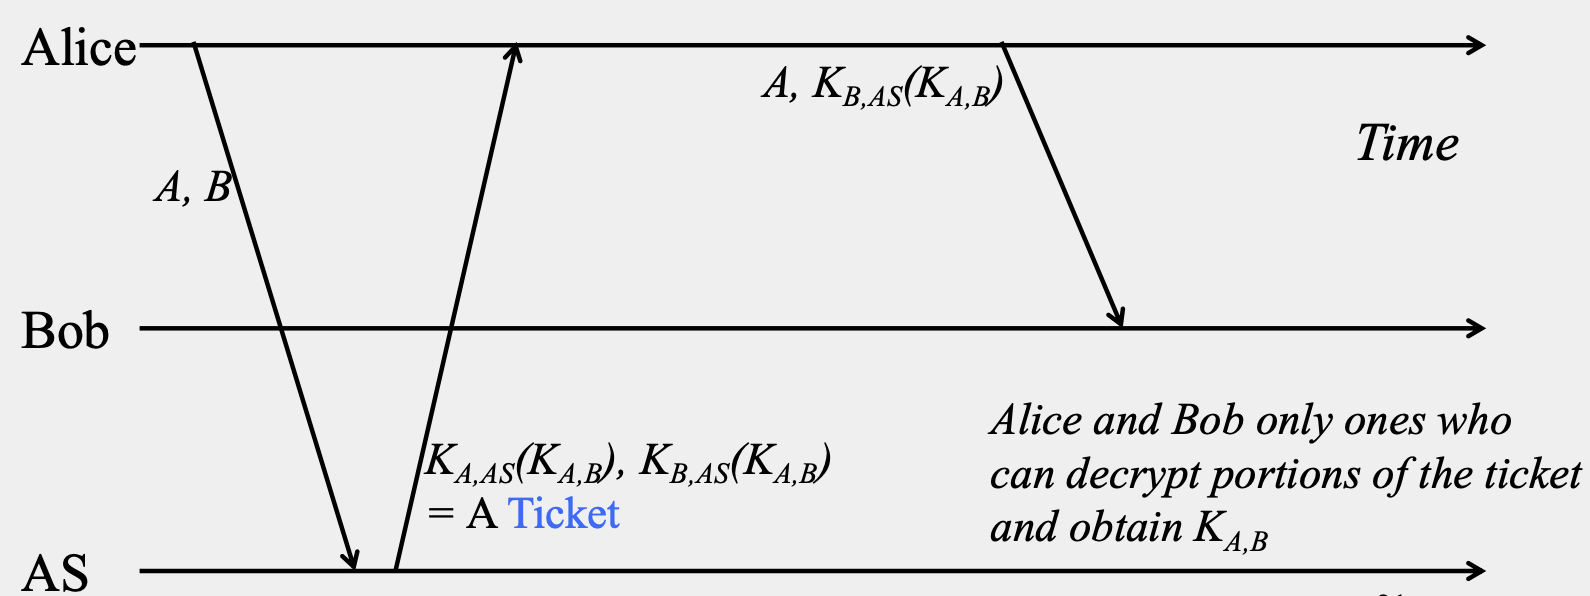
\includegraphics[width=\columnwidth]{indierect.png}
\textbf{Signatures}: authentic, unforgeable, verifiable, non-repudiable: $[M, K_{A\text{priv}}(\text{Hash}(M))]$ (hash for efficiency)
\textbf{Authorization}: Access Control Matrix (large \& sparse),
Access Control Lists (per object, allowed principals/access), Capability Lists (per principal, list of files \& access types)

\end{multicols}
\end{document}
